\documentclass[12pt]{article}
\usepackage{sbc-template}
\usepackage{graphicx,url}
\graphicspath{{figuras/}{imagens/}{./}}
\usepackage[utf8]{inputenc}
\usepackage[brazilian]{babel}
\usepackage{float}
\usepackage{array}
\usepackage{booktabs}
\usepackage[section]{placeins}
\usepackage{amsmath,amssymb}

\sloppy

\title{Predição de ondas de denúncias de violência contra pessoas LGBT, trans e travestis: \\ relação com indicadores municipais no Brasil}

\author{Ana Queiroz da Silva, Natália Metolina, Pedro Henrique Teixeira Soares}

\address{Escola de Artes, Ciências e Humanidades -- Universidade de São Paulo (USP)\\
Rua Arlindo Bétio nº 1000 -- São Paulo -- SP -- Brasil}

  
\begin{document}

\maketitle
     
\begin{resumo}
A violência contra pessoas trans e travestis no Brasil permanece pouco visível nas bases oficiais, que raramente distinguem essa população do conjunto LGBT, e os estudos existentes descrevem tendências nacionais ou estaduais sem antecipar onde as denúncias tendem a se concentrar. Este trabalho integra as denúncias de violência contra pessoas LGBT registradas no Disque 100 entre 2011 e 2022 a indicadores socioeconômicos e institucionais dos 5.565 municípios brasileiros, com o objetivo de identificar municípios com números alarmantes e prever ondas de denúncias. Empregam-se a suavização bayesiana empírica e a estatística de Getis-Ord na identificação de municípios e aglomerados de risco; o modelo endêmico-epidêmico, o LightGBM e o Extra Trees na previsão com horizonte de um ano; regressões binomial e logística na caracterização das vítimas trans; e a série temporal interrompida na avaliação da decisão do Supremo Tribunal Federal (STF) de 2019. Os resultados indicam que as ondas de denúncias são previsíveis e de caráter local, que as denúncias se concentram onde a população LGBT é mais visível e há canais institucionais de denúncia, e que a violência contra pessoas trans é mais grave e mais frequente em espaços públicos. As mudanças no sistema de registro impediram a estimação do efeito da decisão do STF.

\textbf{Palavras-chave:} violência contra população trans; pessoas trans e travestis no Brasil; Disque 100; previsão espaço-temporal; aprendizado de máquina.
\end{resumo}


\clearpage
\section{Introdução}
\label{sec:introducao}

O Brasil é o país com o maior número de assassinatos de pessoas trans, sobretudo de travestis e mulheres trans \cite{marinho_tomazelli_firianelli:2024}. Ainda assim, essa violência é pouco visível nos dados oficiais. Os Censos do Instituto Brasileiro de Geografia e Estatística (IBGE) não registram a identidade de gênero, e estima-se que pessoas trans representem entre 0,1\% e 2\% da população, distribuídas entre as regiões Norte (8\%), Nordeste (26\%), Centro-Oeste (7\%), Sudeste (44\%) e Sul (15\%) \cite{spizziri_eufrasio_lima:2021}. Pessoas trans são aquelas que se identificam com um gênero distinto do atribuído ao nascimento; travestis constituem uma identidade latino-americana de pessoas designadas como do sexo masculino ao nascer que se identificam com o feminino, sem necessariamente se reconhecerem como mulheres \cite{leal_silva_lizzi:2026}. Este trabalho abrange as categorias ``transgênero'', ``travesti'' e ``transexual'', sendo esta última a adotada em bases de dados e documentos oficiais.

A violência, definida como o uso intencional da força ou do poder que possa resultar em lesão, morte, privação ou dano psicológico \cite{marinho_tomazelli_firianelli:2024}, é registrada em bases que raramente distinguem a população trans do conjunto LGBT. No Sistema de Informação de Agravos de Notificação (Sinan), a notificação de violência interpessoal e autoprovocada tornou-se compulsória em 2011, e os campos ``orientação sexual'', ``identidade de gênero'' e ``nome social'' foram incluídos na ficha em 2014. Uma fonte menos explorada é o Disque Direitos Humanos (Disque 100), que recebe denúncias da própria vítima ou de terceiros e mantém, desde 2011, um recorte específico para a população LGBT. Diferentemente do Sinan, restrito aos casos atendidos em serviços de saúde, o Disque 100 também registra violências que raramente geram atendimento, como a discriminação e a violência psicológica. Em 2019, o Supremo Tribunal Federal (STF) enquadrou a transfobia nos crimes previstos na Lei do Racismo (Lei nº 7.716/1989). No campo da saúde, destacam-se o Processo Transexualizador (2008), a Política Nacional de Saúde Integral LGBT (2011) e o direito ao uso do nome social no SUS; o Processo Transexualizador, contudo, está presente em apenas 26 municípios, concentrados nas regiões Sudeste e Sul.

Identificar onde as denúncias são desproporcionalmente elevadas constitui um primeiro passo para conferir visibilidade a essa violência e orientar a ação pública. Nesse contexto, o objetivo deste trabalho é identificar os municípios brasileiros com números alarmantes de denúncias de violência contra pessoas LGBT e, a partir de suas tendências e características, prever em quais deles tendem a ocorrer ondas de denúncias, comparando sempre as vítimas trans ao conjunto da comunidade. O trabalho orienta-se pela seguinte questão: \textit{é possível, a partir de indicadores municipais e do histórico de denúncias, identificar e antecipar os municípios em que a violência contra pessoas LGBT, em especial contra pessoas trans e travestis, é denunciada acima do esperado?} A questão desdobra-se em quatro perguntas: (i) onde se localizam e como se agrupam os municípios com números alarmantes; (ii) se é possível prever ondas de denúncias e qual modelo apresenta melhor desempenho; (iii) se a violência contra pessoas trans difere daquela sofrida pelas demais pessoas LGBT; e (iv) se a decisão do STF alterou o volume de denúncias.


\clearpage
\section{Trabalhos Correlatos}
\label{sec:correlatos}

\subsection{Violência contra pessoas trans nas bases do SUS}

O estudo de \cite{leal_silva_lizzi:2026} analisou 45.715 notificações de violência contra pessoas trans registradas no Sinan entre 2015 e 2023, por meio de um modelo bayesiano hierárquico espaço-temporal de Poisson ajustado por INLA, tendo as 27 unidades da federação como unidade de análise. As vítimas eram majoritariamente mulheres trans (65,3\%), jovens de 19 a 29 anos (36,1\%) e pardas (44,6\%), e a violência física foi a mais frequente (65,9\%). A taxa bruta de notificação passou de 74,3 para 214,0 por 100 mil pessoas trans estimadas entre 2015 e 2023, com valores mais elevados no Sudeste e no Sul, incluindo Minas Gerais, e a autocorrelação espacial foi significativa apenas em 2023. O estudo evidencia que a violência notificada não se distribui aleatoriamente no território, mas não alcança o nível municipal nem propõe previsões.

Em \cite{marinho_tomazelli_firianelli:2024}, foram analisadas as notificações de violência autoprovocada e interpessoal contra pessoas trans de 20 a 59 anos no Sinan, de 2015 a 2022, pelo método de Prais-Winsten. As notificações referentes à população trans corresponderam a 1,7\% do total e apresentaram tendência de queda, ao passo que aumentaram a proporção de municípios notificantes (45,8\%) e as violências autoprovocada e sexual. Os agressores eram majoritariamente homens com vínculo afetivo com a vítima, sobretudo no caso das mulheres trans (43,4\%). A análise descreve a tendência nacional, sem relacionar as notificações a características municipais.

O trabalho de \cite{luis:2025} pareou as notificações de violência contra pessoas trans no Sinan com os óbitos do Sistema de Informações sobre Mortalidade (SIM) entre 2014 e 2022. Das 36.452 notificações, o pareamento recuperou 1.325 óbitos, dos quais 563 (42,5\%) decorreram de causas violentas. O modelo de Poisson indicou maior prevalência de morte violenta entre os mais jovens (razão de prevalência de 4,29 na faixa de 10 a 14 anos), entre as vítimas com registro de lesão autoprovocada (1,50) ou de agressão por arma de fogo (2,00) e quando o óbito ocorreu menos de seis meses após a notificação (2,07). O estudo relaciona violência notificada e mortalidade, porém em nível individual e mediante acesso a dados identificados.

Em conjunto, esses estudos indicam que as notificações ainda não refletem a magnitude da violência contra pessoas trans, em razão da subnotificação e da dificuldade de desagregar essa população do conjunto LGBT, embora o aumento do número de municípios notificantes amplie a visibilidade do problema.

\subsection{Aprendizado de máquina em notificações de violência}

O estudo de \cite{coelho_jiv:2025} aplicou Prophet e Random Forest a 2.635.514 notificações de violência contra a mulher registradas no Sinan (2013--2023), integradas a dados do IBGE, e projetou, a partir de um crescimento médio de 2,26\% ao ano, um aumento de aproximadamente 95\% até 2033. Em \cite{lucca_romero_sbbd:2026}, foram comparados regressão logística regularizada, Random Forest e LightGBM em 2,22 milhões de notificações de violência contra a mulher (2018--2024), com divisão temporal entre treino e teste, na distinção entre violência física, psicológica e sexual. Os modelos não lineares acrescentaram pouco ao modelo linear, o balanceamento de classes prejudicou a calibração das probabilidades e 44,9\% dos casos de violência psicológica não foram identificados, resultado que os autores associam à subnotificação presente na própria base. Esses trabalhos demonstram que algoritmos baseados em árvores de decisão extraem padrões de bases administrativas de violência; contudo, tratam o país de forma agregada ou classificam casos individuais, sem prever a distribuição territorial dos casos, e não foram aplicados à população LGBT (Tabela~\ref{tab:referencia}).

\begin{table}[!htb]
\centering
\caption{Síntese dos trabalhos correlatos e deste trabalho}
\label{tab:referencia}
{\renewcommand{\arraystretch}{1.15}\footnotesize
\begin{tabular}{>{\raggedright\arraybackslash}p{2.5cm} >{\raggedright\arraybackslash}p{3.1cm} >{\raggedright\arraybackslash}p{3.2cm} >{\raggedright\arraybackslash}p{4.4cm}}
\toprule
\textbf{Trabalho} & \textbf{Dados e período} & \textbf{Método} & \textbf{Resultado relevante} \\
\midrule
\cite{leal_silva_lizzi:2026} & Sinan, 2015--2023, 27 UFs & Bayesiano hierárquico (INLA) & Violência não aleatória no território; maiores taxas no Sudeste e no Sul \\
\addlinespace
\cite{marinho_tomazelli_firianelli:2024} & Sinan, 2015--2022 & Prais-Winsten & Trans são 1,7\% das notificações; aumento das violências sexual e autoprovocada \\
\addlinespace
\cite{luis:2025} & Sinan e SIM, 2014--2022 & Pareamento e Poisson & 42,5\% dos óbitos pareados por causa violenta; risco maior entre jovens \\
\addlinespace
\cite{coelho_jiv:2025} & Sinan e IBGE, 2013--2023 (mulheres) & Prophet e Random Forest & Projeção de cerca de +95\% até 2033 \\
\addlinespace
\cite{lucca_romero_sbbd:2026} & Sinan, 2018--2024 (mulheres) & Logística, Random Forest e LightGBM & Não lineares acrescentam pouco; 44,9\% da violência psicológica não identificada \\
\midrule
\textbf{Este trabalho} & Disque 100, IBGE, MUNIC e SUS, 2011--2022, 5.565 municípios & Bayes empírico, Getis-Ord, endêmico-epidêmico, LightGBM, Extra Trees e série interrompida & Municípios alarmantes e previsão de ondas, comparando vítimas trans e LGBT \\
\bottomrule
\end{tabular}}
\end{table}

\subsection{Vigilância de surtos aplicada ao território}

A previsão da concentração territorial das denúncias aproxima-se de um problema clássico da vigilância epidemiológica, que acompanha contagens de casos por área e período com o objetivo de detectar surtos precocemente. Em \cite{farrington:1996}, foi proposto um algoritmo que compara a contagem de cada período com um limiar estimado a partir do histórico e emite um alerta quando esse limiar é ultrapassado, adotado na vigilância de doenças infecciosas na Inglaterra e no País de Gales. O modelo endêmico-epidêmico \cite{held_hohle_hofmann:2005} estendeu essa abordagem a múltiplas áreas: o número esperado de casos em cada área é decomposto em um componente endêmico, associado às características locais, um componente autorregressivo, dependente dos casos recentes na própria área, e um componente espacial, dependente dos casos nas áreas vizinhas, o que permite avaliar se um surto se propaga pelo território. Em mapas de pequenas áreas, a suavização bayesiana empírica \cite{marshall:1991} evita que municípios pouco populosos apresentem valores extremos por variação aleatória, e a estatística local de Getis-Ord \cite{getis_ord:1992} identifica aglomerados de valores elevados.

Embora desenvolvidas para doenças, essas ferramentas aplicam-se a problemas de mesma estrutura: contagens raras, distribuídas de forma desigual entre áreas e sujeitas a elevações abruptas. Nos trabalhos revisados, tais métodos não foram empregados na análise de denúncias de violência contra pessoas LGBT, e nenhum estudo avaliou, com dados de denúncia, o efeito da decisão do STF. Este trabalho articula as três vertentes discutidas nesta seção: aplica a lógica da vigilância de surtos à população que os estudos com dados do SUS apontam como mais exposta e formula a questão preditiva ainda não abordada pelos estudos com aprendizado de máquina, comparando modelos estatísticos e de aprendizado de máquina em vez de adotar um deles a priori.


\clearpage
\section{Metodologia}
\label{sec:metodologia}

Trata-se de um estudo ecológico, cuja unidade de análise é o par município-ano: para cada um dos 5.565 municípios e cada ano entre 2011 e 2022, foram reunidas as denúncias de violência contra pessoas LGBT e características municipais. As quatro análises convergem para a questão central: \textbf{onde a violência denunciada é alarmante e quais municípios tendem a apresentar ondas de denúncias}.

\subsection{Coleta de dados}

\textbf{Denúncias.} A fonte é o Disque Direitos Humanos (Disque 100), mantido pela Ouvidoria Nacional de Direitos Humanos. Foram utilizadas as denúncias de janeiro de 2011 a dezembro de 2022 cuja vítima pertence ao grupo ``população LGBTQIA+'' (50.045 linhas). De cada denúncia, foram extraídos data, município, perfil da vítima, tipo de violação, local, relação com o agressor e, a partir de 2020, o denunciante e o canal utilizado.

\textbf{Características municipais.} Os dados municipais foram obtidos de fontes oficiais por meio de script, o que garante a reprodutibilidade da coleta (Tabela~\ref{tab:fontes}). As coordenadas de cada município definiram seus 10 vizinhos mais próximos. A última coluna da tabela indica o papel de cada fonte nos resultados; a proporção de domicílios com casal do mesmo sexo foi adotada como aproximação da população LGBT visível de cada município.

\begin{table}[H]
\centering
\caption{Fontes de dados, variáveis municipais e seu papel nos resultados}
\label{tab:fontes}
{\renewcommand{\arraystretch}{1.2}\small
\begin{tabular}{>{\raggedright\arraybackslash}p{4.4cm} >{\raggedright\arraybackslash}p{3.7cm} >{\raggedright\arraybackslash}p{1.9cm} >{\raggedright\arraybackslash}p{3.3cm}}
\toprule
\textbf{Variável} & \textbf{Fonte} & \textbf{Período} & \textbf{Papel nos resultados} \\
\midrule
Denúncias contra pessoas LGBT & Disque 100 & 2011--2022 & variável prevista; histórico é o principal preditor \\
Casais do mesmo sexo; densidade & IBGE, Censo 2022 & 2022 & fatores mais fortes (mais denúncias) \\
População residente & IBGE & 2011--2022 & base do valor esperado \\
Cor ou raça; 15 a 29 anos & IBGE, Censos 2010 e 2022 & 2010, 2022 & pretos e pardos: menos denúncias \\
Políticas de direitos humanos e LGBT & IBGE, MUNIC & 2014, 2019, 2023 & ouvidoria: mais denúncias \\
PIB, renda, Gini e homicídios & IBGE, Atlas DH, Atlas da Violência & 2010--2022 & sem efeito \\
Processo Transexualizador & SUS (SIA/SIH) & 2008--2026 & sem efeito \\
\bottomrule
\end{tabular}}
\end{table}

\subsection{Limpeza e Normalização dos Dados}

O sistema de registro do Disque 100 foi alterado três vezes no período (2011--2019, primeiro semestre de 2020 e a partir de julho de 2020); no formato mais recente, cada linha corresponde a uma violação, e não a uma denúncia. Foram removidas 561 linhas duplicadas e agrupadas as linhas referentes à mesma denúncia e vítima, resultando em \textbf{27.441 registros}. As colunas equivalentes dos três formatos foram unificadas, respostas como ``não informado'' foram reunidas na categoria ``desconhecido'' e as cerca de 240 descrições de violação foram agrupadas em nove tipos. Entre julho de 2020 e junho de 2022, o formulário não permitia o registro da identidade trans; nesse intervalo, a variável foi tratada como ausente, e não como zero. Do total de registros, 97,6\% foram associados ao código do município (2.070 municípios), e o painel município-ano foi completado com zeros nas combinações sem denúncia. Os valores monetários foram deflacionados para reais de 2022, os dados censitários foram interpolados entre 2010 e 2022, e as sete questões comuns às edições da MUNIC compuseram um índice de política LGBT de 0 a 4. Por fim, as variáveis categóricas foram codificadas em variáveis binárias, e as variáveis de elevada assimetria, como população e PIB, foram transformadas em logaritmo e padronizadas.

\subsection{Análise Estatística das Notificações de Violência e Correlação entre Variáveis}

Em 91\% das combinações de município e ano não há denúncias, o que requer modelos adequados a contagens com excesso de zeros, e o volume nacional varia por razões administrativas do Disque 100. Por isso, o total nacional foi tratado como dado, e a modelagem concentrou-se na distribuição territorial das denúncias. Para cada município e ano, calculou-se o \textbf{valor esperado}, isto é, o número de denúncias que o município receberia caso sua participação no total nacional fosse proporcional à sua população.

\textbf{Análise 1 --- municípios alarmantes e previsão de ondas.} A razão entre denúncias observadas e esperadas (risco relativo) foi estimada com \textbf{suavização bayesiana empírica} \cite{marshall:1991}, de modo a evitar que uma única denúncia em um município pequeno produza um falso alarme; considerou-se \textbf{alarmante} o município com probabilidade superior a 95\% de estar acima do esperado. A estatística de \textbf{Getis-Ord} \cite{getis_ord:1992} foi utilizada para identificar aglomerados de municípios alarmantes. Na previsão das denúncias do ano seguinte, foram comparados três modelos: o \textbf{endêmico-epidêmico} \cite{held_hohle_hofmann:2005}, que decompõe o volume esperado em componente estrutural, inércia do próprio histórico e propagação a partir dos vizinhos; o \textbf{LightGBM} \cite{ke:2017}, baseado em árvores de decisão com \textit{boosting}; e o \textbf{Extra Trees} \cite{geurts:2006}, da família das florestas aleatórias. Os modelos foram comparados a três referências simples: distribuição proporcional à população, repetição da participação histórica do município e repetição do valor do ano anterior. Definiu-se \textbf{onda} como um ano com ao menos 5 denúncias e ao menos o dobro do valor esperado; um município entra em \textbf{alerta} quando supera o percentil 95 da distribuição prevista pelo modelo \cite{farrington:1996}.

\textbf{Análises 2 e 3 --- vítimas trans.} Uma \textbf{regressão binomial} identificou as características municipais associadas à proporção de vítimas trans entre as denúncias LGBT, com comparação entre municípios no mesmo ano. Uma \textbf{regressão logística}, comparada ao LightGBM, identificou as características da denúncia associadas à vítima trans (16.467 registros).

\textbf{Análise 4 --- decisão do STF.} Uma \textbf{série temporal interrompida} \cite{bernal:2017} comparou as denúncias mensais posteriores a junho de 2019 com a tendência anterior, com controle da pandemia, das mudanças de sistema e da sazonalidade. Um \textbf{teste de placebo} repetiu a análise para cada mês de 2018 e 2019, verificando se outra data explica melhor a mudança.

Os efeitos são expressos como \textbf{razão de taxas} (RR) ou \textbf{razão de chances}; intervalos de confiança de 95\% (IC 95\%) que incluem o valor 1 indicam ausência de evidência de efeito.

\subsection{Protocolo de validação, métricas e reprodução}

A avaliação reproduz as condições de uso: em cada rodada, os modelos são treinados com todos os anos anteriores ao ano previsto e aplicados aos 5.565 municípios do ano seguinte, sem qualquer ajuste com os dados de teste (Tabela~\ref{tab:rodadas}). O LightGBM utiliza perda Tweedie (potência 1,3), adequada a contagens com excesso de zeros, taxa de aprendizado de 0,03, 15 folhas, mínimo de 60 observações por folha e o logaritmo do valor esperado como termo fixo (\textit{offset}); o número de árvores é definido por parada antecipada (até 2.000, com interrupção após 100 iterações sem melhora no último ano de treino), e o modelo é então retreinado com todos os anos. O Extra Trees utiliza 300 árvores, critério de Poisson e mínimo de 20 observações por folha; o endêmico-epidêmico é estimado por máxima verossimilhança. A semente aleatória é 42.

\begin{table}[H]
\centering
\caption{Rodadas da validação temporal: cada linha treina com os anos anteriores e prevê o ano indicado}
\label{tab:rodadas}
{\renewcommand{\arraystretch}{1.0}\footnotesize
\begin{tabular}{c c r r r r}
\toprule
\textbf{Ano previsto} & \textbf{Anos de treino} & \textbf{Obs. de treino} & \textbf{Sem denúncia} & \textbf{Ondas} & \textbf{Árvores} \\
\midrule
2016 & 2012--2015 & 22.260 & 92,7\% & 56 & 155 \\
2017 & 2012--2016 & 27.825 & 91,3\% & 59 & 130 \\
2018 & 2012--2017 & 33.390 & 92,5\% & 42 & 139 \\
2019 & 2012--2018 & 38.955 & 94,2\% & 42 & 352 \\
2020 & 2012--2019 & 44.520 & 93,4\% & 50 & 131 \\
2021 & 2012--2020 & 50.085 & 93,8\% & 31 & 942 \\
2022 & 2012--2021 & 55.650 & 85,8\% & 52 & 757 \\
\bottomrule
\multicolumn{6}{p{12.5cm}}{\footnotesize 5.565 municípios por ano previsto. Sem denúncia: municípios com zero registro. Árvores: escolhidas pela parada antecipada do LightGBM.}
\end{tabular}}
\end{table}

A métrica principal é o desvio de Poisson médio, que mede o erro de previsão de contagens sem que os municípios mais populosos dominem a avaliação, como ocorreria com o erro quadrático; o ganho de cada modelo corresponde à redução desse desvio em relação à referência proporcional à população. Por serem raras (menos de 1\% dos municípios por ano), as ondas foram avaliadas pela precisão entre os 20 municípios apontados como mais prováveis e pela precisão média, métricas mais informativas que a acurácia em classes desbalanceadas \cite{saito_rehmsmeier:2015}. As análises foram implementadas em Python 3.13 (\textit{statsmodels} 0.15, \textit{scikit-learn} 1.9, \textit{LightGBM} 4.7, \textit{SHAP} e \textit{PySAL}); com a semente fixa, a execução reproduz os mesmos resultados.


\clearpage
\section{Resultados e Discussão dos Resultados}
\label{sec:resultados}

\subsection{Panorama das denúncias}

Entre 2011 e 2022, o Disque 100 registrou 27.441 denúncias de violência contra pessoas LGBT, provenientes de 2.070 municípios (37\% do total). A maioria das vítimas era do gênero masculino (62\%), homossexual (68\%) e jovem (47\% entre 18 e 29 anos); em 28\% dos casos, a raça/cor não foi informada. A violência psicológica esteve presente em 79\% dos registros, seguida da discriminação (53\%) e da agressão física (32\%). A partir de 2020, 70\% das denúncias foram realizadas pela própria vítima, quase todas por telefone.

As principais variações do total nacional coincidem com mudanças administrativas, e não com alterações conhecidas na violência (Figura~\ref{fig:serie}): o volume reduziu-se após a troca de sistema em julho de 2020 e multiplicou-se por aproximadamente 4,5 com o novo formulário de julho de 2022. Por esse motivo, as análises consideram a \textit{distribuição} das denúncias entre os municípios, e não o total nacional.

\begin{figure}[!htb]
\centering
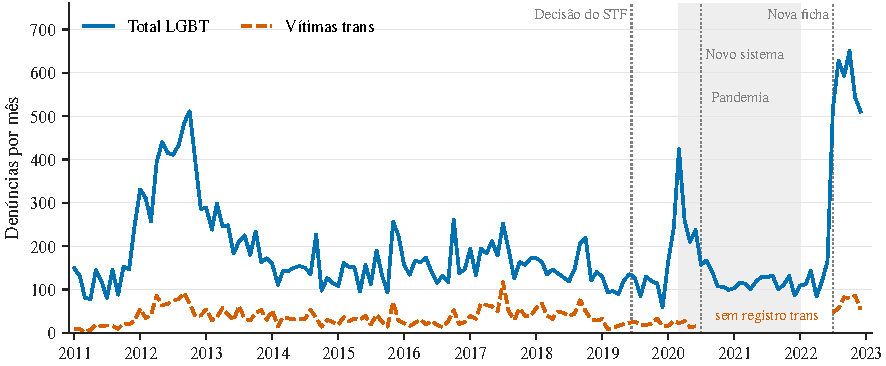
\includegraphics[width=\textwidth]{fig1_serie_mensal.pdf}
\caption{Denúncias mensais de violência contra pessoas LGBT (linha contínua azul) e contra vítimas trans (linha tracejada vermelha), 2011--2022. As linhas verticais pontilhadas marcam a decisão do STF e as mudanças no sistema de registro; a faixa cinza, a pandemia. Fonte: Disque 100 (ONDH/MDHC).}
\label{fig:serie}
\end{figure}

\subsection{Onde estão os municípios alarmantes?}

Os municípios alarmantes localizam-se, em sua maioria, fora dos grandes centros e concentram-se em poucas regiões. Um número elevado de denúncias não implica, por si só, risco elevado: os 50 municípios com mais registros concentram metade do total, mas São Paulo, com o maior número absoluto, situa-se apenas 31\% acima do esperado para seu porte. Após o controle do tamanho populacional e da variação aleatória, \textbf{141 municípios apresentaram números alarmantes em 2020--2022}, dos quais 83 possuem menos de 100 mil habitantes. Os valores mais extremos foram observados em Ubaporanga (MG, quase 30 vezes o esperado), Itaporanga (PB, 25), Cabo Frio (RJ, 17), Barbacena (MG, 10) e Campos dos Goytacazes (RJ, 8). Esses municípios formam \textbf{61 aglomerados de alto risco}, situados na Zona da Mata e no Sul de Minas Gerais, na região metropolitana do Rio de Janeiro, no interior de São Paulo, em Goiás e no entorno de João Pessoa (Figura~\ref{fig:mapa}).

\begin{figure}[!htb]
\centering
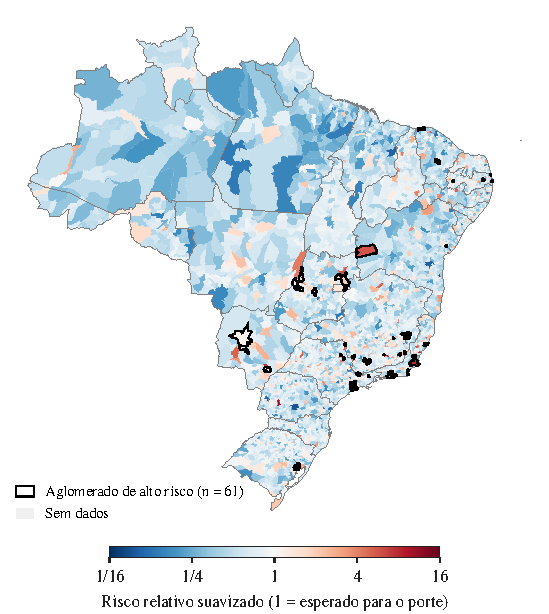
\includegraphics[width=0.62\textwidth]{fig3_mapa_risco.pdf}
\caption{Risco relativo suavizado de denúncias por município, 2020--2022. Vermelho: mais denúncias do que o esperado para o porte; azul: menos; branco: o esperado. O contorno preto marca os aglomerados de alto risco (Getis-Ord, $p<0{,}05$). Fonte: Disque 100 e IBGE.}
\label{fig:mapa}
\end{figure}

\subsection{É possível prever as ondas?}

Sim. Os três modelos apresentaram desempenho superior à distribuição proporcional à população, e as referências simples tiveram desempenho inferior (Tabela~\ref{tab:validacao}). O LightGBM obteve o melhor resultado, com erro 16,7\% menor que o da referência, seguido pelo modelo endêmico-epidêmico (14,6\%). A repetição do ano anterior foi a pior estratégia, pois o número de denúncias de um município varia consideravelmente entre anos, e o histórico só contribui quando combinado às características municipais. O principal ganho refere-se às ondas: dos 20 municípios apontados anualmente pelo LightGBM como mais prováveis, 37\% efetivamente apresentaram onda, contra 15\% na referência populacional. Como apenas cerca de 47 dos 5.565 municípios apresentam onda a cada ano (0,85\%), uma seleção aleatória de 20 municípios teria precisão inferior a 1\%, de modo que o acerto do modelo é mais de 40 vezes superior ao acaso. A precisão permanece distante de 100\% porque a maior parte das ondas é transitória e depende da iniciativa de denunciar; o modelo destina-se, portanto, à priorização da atenção, e não à emissão de alertas determinísticos.

\begin{table}[!htb]
\centering
\caption{Desempenho dos modelos na previsão um ano à frente (média de 2016 a 2022)}
\label{tab:validacao}
{\renewcommand{\arraystretch}{1.15}\small
\begin{tabular}{p{4.6cm} p{2.6cm} p{2.6cm} p{3.0cm}}
\toprule
\textbf{Modelo} & \textbf{Redução do erro em relação à população} & \textbf{Acerto das 50 maiores cidades} & \textbf{Acerto entre as 20 cidades apontadas para onda} \\
\midrule
LightGBM & 16,7\% & 66\% & 37\% \\
Endêmico-epidêmico & 14,6\% & 63\% & 31\% \\
Extra Trees & 11,3\% & 63\% & 31\% \\
Só população (referência) & -- & 63\% & 15\% \\
Fatia histórica da cidade & $-$14,7\% & 61\% & 29\% \\
Repetir o ano anterior & $-$35,8\% & 55\% & 26\% \\
\bottomrule
\end{tabular}}
\end{table}

\subsection{O que está associado a mais denúncias?}

As denúncias associam-se à visibilidade da população LGBT e à existência de canais institucionais de denúncia. O fator de maior magnitude foi a proporção de domicílios com casais do mesmo sexo, a melhor aproximação disponível da população LGBT visível: o aumento de um desvio-padrão nesse indicador associou-se a 13\% mais denúncias (Tabela~\ref{tab:coef}). A densidade demográfica apresentou efeito semelhante, e a existência de ouvidoria municipal de direitos humanos associou-se a 23\% mais denúncias. Municípios com maior proporção de pessoas pretas e pardas registraram 8\% menos denúncias, e as regiões Norte e Sul, menos denúncias que o Sudeste. Renda, PIB, desigualdade, homicídios, índice de política LGBT e Processo Transexualizador não apresentaram associação com o volume de denúncias.

\begin{table}[!htb]
\centering
\caption{Características associadas a mais (RR $>$ 1) ou menos (RR $<$ 1) denúncias do que o esperado para o porte do município}
\label{tab:coef}
{\renewcommand{\arraystretch}{1.1}\small
\begin{tabular}{p{6.8cm} c c c}
\toprule
\textbf{Característica} & \textbf{RR} & \textbf{IC 95\%} & \textbf{Há efeito?} \\
\midrule
Casais do mesmo sexo (por desvio-padrão) & 1,13 & 1,08--1,18 & sim \\
Densidade demográfica (por desvio-padrão) & 1,12 & 1,07--1,18 & sim \\
População (por desvio-padrão) & 1,08 & 1,02--1,15 & sim \\
Pretos e pardos (por desvio-padrão) & 0,92 & 0,86--0,98 & sim \\
Tem ouvidoria de direitos humanos & 1,23 & 1,10--1,37 & sim \\
Região Centro-Oeste (em relação ao Sudeste) & 1,36 & 1,17--1,57 & sim \\
Região Sul & 0,72 & 0,64--0,81 & sim \\
Região Norte & 0,58 & 0,48--0,70 & sim \\
Renda domiciliar por pessoa & 1,01 & 0,92--1,10 & não \\
Taxa de homicídios no ano anterior & 0,99 & 0,94--1,03 & não \\
Índice de política LGBT (MUNIC) & 0,99 & 0,96--1,01 & não \\
Processo Transexualizador ativo & 0,71 & 0,34--1,46 & não \\
\bottomrule
\multicolumn{4}{p{12cm}}{\footnotesize Modelo endêmico-epidêmico, 2012--2022. Também incluídos, sem efeito: PIB por pessoa, Gini, população de 15 a 29 anos, estrutura municipal de direitos humanos, capital e Nordeste.}
\end{tabular}}
\end{table}

As ondas têm caráter local. Das denúncias esperadas pelo modelo endêmico-epidêmico, 74\% decorrem das características do próprio município, 26\% da inércia de seu histórico e apenas 0,3\% dos municípios vizinhos. A cada ano, entre 22 e 52 municípios entraram em alerta, e um município em alerta apresentou probabilidade quase seis vezes maior de permanecer em alerta no ano seguinte.

\subsection{Por que confiar na previsão?}

O modelo aprende de forma controlada, seu ganho se mantém em todos os anos avaliados e as relações aprendidas coincidem com as do modelo estatístico. O LightGBM constrói árvores de decisão sequencialmente, cada uma corrigindo os erros das anteriores. Nas curvas de aprendizado (Figura~\ref{fig:curvas}), o erro no treino decresce continuamente, enquanto o erro no ano reservado para validação decresce até um mínimo e depois volta a aumentar (até 11\% acima do mínimo); a interrupção do treino nesse ponto evita o sobreajuste.

\begin{figure}[!htb]
\centering
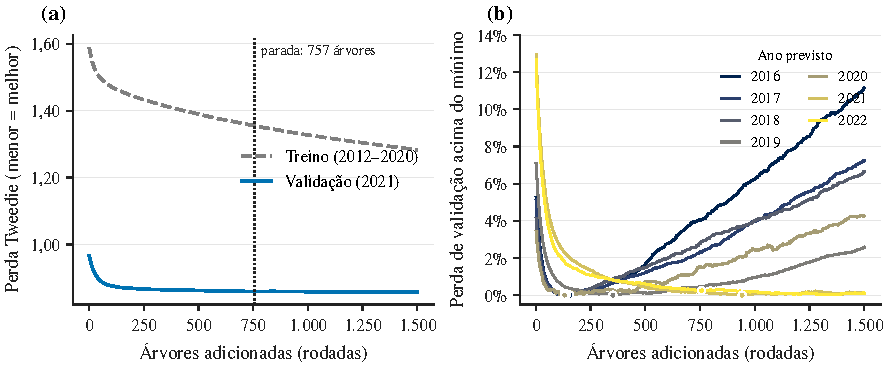
\includegraphics[width=\textwidth]{fig5_curvas_aprendizado.pdf}
\caption{Aprendizado do LightGBM ao longo das árvores. (a) Previsão de 2022: erro no treino (cinza tracejado) e no ano reservado para conferência (azul); a linha pontilhada marca onde o treino parou. (b) Erro de conferência acima do seu mínimo, para cada ano previsto; os círculos marcam o ponto de parada. Fonte: Disque 100 e IBGE.}
\label{fig:curvas}
\end{figure}

Os ganhos mantêm-se na reamostragem dos municípios, e os três modelos superam a referência em todos os anos (Tabela~\ref{tab:robustez}). A vantagem do LightGBM sobre o endêmico-epidêmico é pequena (2,1 pontos percentuais), mas repetiu-se em seis dos sete anos, e o ganho variou entre 15,7\% e 17,3\% sob diferentes hiperparâmetros. Na ablação, a informação dos municípios vizinhos acrescentou apenas 0,15 ponto, o que confirma a ausência de propagação espacial das ondas. As previsões são calibradas (o modelo previu 96\% das denúncias ocorridas) e úteis para a priorização: com o monitoramento de 1\% dos municípios por ano, os selecionados pelo LightGBM concentraram 31\% das ondas, contra 22\% na seleção pela população (Figura~\ref{fig:calib}). Os valores SHAP indicam que o modelo, sem especificação prévia, aprendeu as relações da Tabela~\ref{tab:coef}.

\begin{table}[!htb]
\centering
\caption{Confiabilidade e custo dos modelos de previsão (validação de 2016 a 2022)}
\label{tab:robustez}
{\renewcommand{\arraystretch}{1.1}\small
\begin{tabular}{>{\raggedright\arraybackslash}p{5.0cm} >{\raggedright\arraybackslash}p{3.0cm} >{\raggedright\arraybackslash}p{2.4cm} >{\raggedright\arraybackslash}p{2.4cm}}
\toprule
\textbf{Modelo} & \textbf{Redução do erro (IC 95\%)} & \textbf{Anos melhor que a referência} & \textbf{Tempo por rodada} \\
\midrule
LightGBM & 16,7\% (13,3--20,3) & 7 de 7 & 0,5 a 4 s \\
Endêmico-epidêmico & 14,6\% (11,0--18,7) & 7 de 7 & 2 a 4,5 s \\
Extra Trees & 11,3\% (6,9--15,2) & 7 de 7 & 2,5 a 6,5 s \\
\midrule
\textbf{Informações usadas pelo LightGBM} & \textbf{Redução média por ano} & & \\
\midrule
Só características do município & 14,0\% & & \\
Só histórico da cidade & 14,1\% & & \\
Características e histórico & 16,7\% & & \\
Completo (com cidades vizinhas) & 16,9\% & & \\
\bottomrule
\multicolumn{4}{p{13cm}}{\footnotesize IC por reamostragem dos municípios (2.000 vezes). Na ablação, a redução é a média dos ganhos de cada ano, por isso o modelo completo difere 0,2 ponto da primeira parte. Tempos em computador comum, sem placa de vídeo.}
\end{tabular}}
\end{table}

\begin{figure}[!htb]
\centering
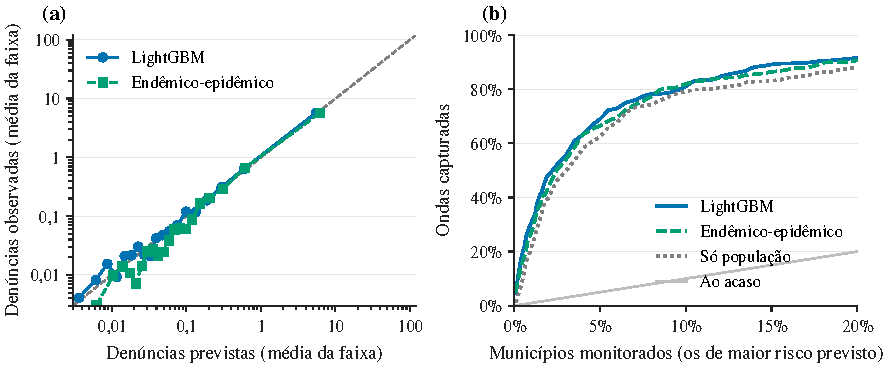
\includegraphics[width=\textwidth]{fig8_calibracao_captura.pdf}
\caption{(a) Calibração: denúncias previstas e observadas, por faixa de previsão (escala log); a linha tracejada indica previsão perfeita. (b) Percentual das 332 ondas de 2016 a 2022 capturado quando se monitoram os municípios de maior risco previsto; a linha cinza indica a escolha ao acaso. Previsões fora da amostra. Fonte: Disque 100 e IBGE.}
\label{fig:calib}
\end{figure}

\subsection{A violência contra pessoas trans é diferente?}

Sim: a violência contra pessoas trans é mais grave, mais frequente em espaços públicos e registrada de forma mais incompleta. Nos períodos com registro da identidade de gênero (ausente entre julho de 2020 e junho de 2022), 18\% das denúncias LGBT referiam-se a vítimas trans (4.406 de 24.151), número insuficiente para previsões em nível municipal; por isso, essa violência foi analisada por sua proporção e seu perfil. Na comparação entre municípios no mesmo ano, essa proporção foi maior no Nordeste (chance 54\% superior à do Sudeste) e menor em municípios mais densos e com maior proporção de pessoas pretas e pardas. Os municípios alarmantes não diferem dos demais nesse aspecto (17\% contra 19\%), o que indica que as ondas atingem a comunidade LGBT como um todo.

Em violações contra a vida, a chance de a vítima ser trans é três vezes maior; essa chance também é maior na violência sexual (1,7) e física (1,4), em vias públicas e quando o agressor é desconhecido (1,7) ou profissional e agente de instituição (2,3) (Figura~\ref{fig:perfil}). Esses registros são também mais incompletos: a raça/cor está ausente em 30\% deles, contra 16\% nos demais. O modelo distingue os dois grupos de forma moderada (AUC de 0,71), e o LightGBM não superou a regressão logística.

\begin{figure}[!htb]
\centering
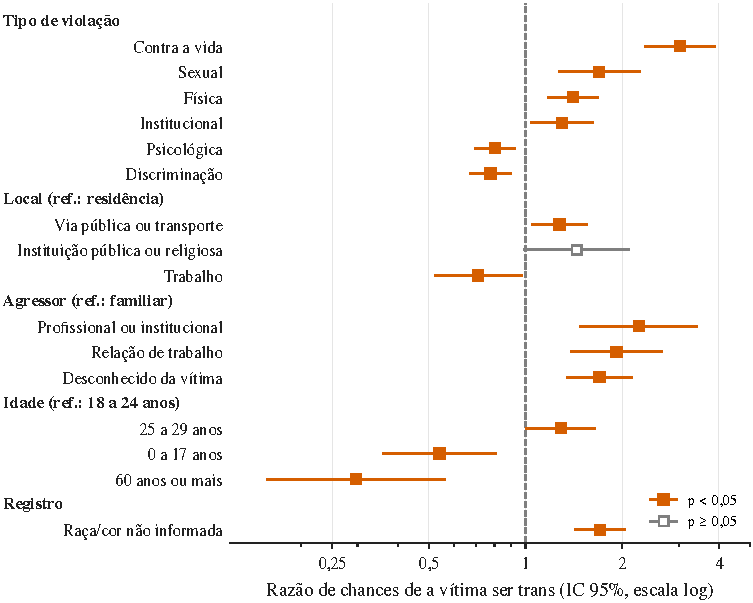
\includegraphics[width=0.85\textwidth]{fig4_perfil_trans.pdf}
\caption{Quanto cada característica da denúncia aumenta (à direita de 1) ou reduz (à esquerda de 1) a chance de a vítima ser trans. Quadrados cheios: efeito estatisticamente significativo ($p<0{,}05$); quadrados vazados em cinza: sem efeito. As linhas horizontais mostram o intervalo de confiança de 95\%. Fonte: Disque 100 (ONDH/MDHC).}
\label{fig:perfil}
\end{figure}

\subsection{A decisão do STF mudou as denúncias?}

Não foi possível identificar efeito. A decisão do STF que enquadrou a transfobia na Lei do Racismo, de 13 de junho de 2019, não foi seguida de alteração no total de denúncias LGBT (RR 0,98; IC 95\%: 0,67--1,43). As denúncias com vítima trans reduziram-se em 48\%, mas o teste de placebo indicou que a queda teve início em fevereiro de 2019, quatro meses antes da decisão, simultaneamente a uma mudança no registro da categoria ``travesti''. Com apenas 13 meses de registros trans posteriores à decisão, seu efeito não pode ser estimado. As mudanças administrativas, por outro lado, tiveram grande impacto: a troca de sistema reduziu o volume em 59\%, e o novo formulário o multiplicou por 4,5.

\subsection{Relação com a literatura e limitações}

Os estudos citados utilizam o Sinan, que registra atendimentos em saúde, enquanto este trabalho utiliza denúncias; por isso, os resultados são comparados quanto à direção, e não à magnitude. A participação de vítimas trans no Disque 100 (18\% das denúncias LGBT) é muito superior à observada no Sinan, em que pessoas trans representam 1,7\% de todas as notificações de violência \cite{marinho_tomazelli_firianelli:2024}. A cobertura territorial é semelhante: 45,8\% dos municípios já notificaram violência contra pessoas trans no Sinan \cite{marinho_tomazelli_firianelli:2024}, e 37\% registraram ao menos uma denúncia LGBT no Disque 100, ou seja, a maioria dos municípios ainda não aparece em nenhuma das duas bases. O perfil é convergente: no Sinan predominam mulheres trans jovens, a violência física e o aumento da violência sexual \cite{leal_silva_lizzi:2026,marinho_tomazelli_firianelli:2024}, e, neste trabalho, as vítimas trans são mais jovens e têm maior chance de sofrer violência física, sexual e contra a vida, em consonância com a maior mortalidade violenta entre pessoas trans jovens \cite{luis:2025}. A divergência refere-se ao agressor: no Sinan, predominam parceiros com vínculo afetivo \cite{marinho_tomazelli_firianelli:2024}, ao passo que no Disque 100 as vítimas trans distinguem-se pela violência de desconhecidos e de agentes institucionais, o que pode refletir o tipo de caso recebido por cada canal.

No território, \cite{leal_silva_lizzi:2026} identificaram as maiores taxas no Sudeste e no Sul, com Minas Gerais entre os estados de valores mais elevados, e autocorrelação espacial fraca; os aglomerados em Minas Gerais e a contribuição praticamente nula dos vizinhos confirmam esse padrão em nível municipal. No mesmo estudo, 44,6\% das vítimas eram pardas, enquanto, neste trabalho, os municípios com maior proporção de pessoas pretas e pardas denunciam menos que o esperado; em conjunto, os resultados sugerem subnotificação justamente onde a violência é mais incidente, ainda que um seja medido em nível individual e o outro em nível municipal. Em linha com \cite{lucca_romero_sbbd:2026}, o aprendizado de máquina não superou a regressão logística na classificação de casos individuais; na previsão de contagens municipais com histórico, entretanto, o LightGBM superou o modelo estatístico, o que demonstra a aplicabilidade da lógica de vigilância de surtos \cite{held_hohle_hofmann:2005} a denúncias de violência. Diferentemente de \cite{coelho_jiv:2025}, não se projetou o volume nacional, uma vez que, no Disque 100, ele depende de mudanças administrativas. Quanto ao STF, nenhum dos estudos revisados avaliou a decisão com dados de denúncia; o resultado nulo indica que a estimação de seu efeito requer séries com registro estável da identidade de gênero.

As conclusões estão sujeitas a seis limitações principais. Primeiro, o Disque 100 mede denúncias, e não a ocorrência de violência, e a subnotificação pode variar entre municípios. Segundo, o delineamento é ecológico: as associações referem-se a municípios, e não a indivíduos, e não implicam causalidade. Terceiro, a identidade trans não foi registrada entre julho de 2020 e junho de 2022, e há apenas 13 meses de registros trans posteriores à decisão do STF. Quarto, a proporção de casais do mesmo sexo está disponível apenas no Censo de 2022, e outras variáveis censitárias foram interpoladas. Quinto, a previsão trata o volume nacional do ano seguinte como conhecido. Sexto, os dados encerram-se em 2022, e as estimativas para 2023 ainda não foram verificadas.


\clearpage
\section{Conclusão}
\label{sec:conclusao}

Este trabalho investigou se é possível identificar e antecipar os municípios em que a violência contra pessoas LGBT, em especial contra pessoas trans e travestis, é denunciada acima do esperado, e a resposta é afirmativa. (i) Os 141 municípios alarmantes não se restringem aos grandes centros e concentram-se em aglomerados, sobretudo em Minas Gerais, no Rio de Janeiro e no entorno de João Pessoa. (ii) As ondas são previsíveis: o LightGBM apresentou o melhor desempenho e, com o monitoramento de 1\% dos municípios, concentrou aproximadamente um terço delas; as denúncias são mais frequentes onde a população LGBT é mais visível e há ouvidoria, e menos frequentes onde há maior proporção de pessoas pretas e pardas, padrão compatível com subnotificação. (iii) A violência contra pessoas trans é mais grave e mais frequente em espaços públicos, inclusive quando praticada por agentes institucionais, e seus registros são os mais incompletos. (iv) O efeito da decisão do STF não pôde ser estimado, uma vez que as mudanças no registro superaram o efeito do marco legal. Como trabalhos futuros, propõem-se a manutenção de um campo estável de identidade de gênero no Disque 100, o cruzamento das denúncias com o Sinan e o SIM e a validação da previsão com dados de 2023 em diante.


\clearpage
\bibliographystyle{sbc}
\bibliography{sbc-template,referencias_metodo}

\end{document}
